\section{Proof synthesis}
\label{sec:synthesis}

\subsection{Front-end proof to kernel proof}

In the front a backward proof is characterized by an initial proof goal and a sequence of tactics to apply such that they eventually reduce the goal to nil. Forward proofs in the front are much more concise as they are the result of a single step; e.g. a forward rule application. As stated in the requirements, we would like to be able to translate these two proofs into kernel proofs. We describe how this process works in this section. Note that since we are not that much interested in the final shape of the proof, it is not strictly speaking a one-to-one translation but rather a synthesis (or a reconstruction) process. Such a relaxation allows us for instance to optimize the proof.

For backward proofs the first step is to reverse the order of the tactics and successive states. This is necessary as kernel proofs must be constructed forward; any changes to existing steps would require a complete reorganization of the proof. At the same time, we should also label each distinct proof goal as they will either represent an individual proof step or an import in the final kernel proof. This mechanism is achieved thanks to the \textbf{shadow proof state}, which associates identifiers to the goals in the proof state. That way, when a proof goal is transformed into subgoals we can recover the ids of the premises and the current step. Similarly, when proof goals are reordered we should update the shadow state accordingly to reflect the new order.

Then, we can proceed with the reconstruction of the kernel proof. Recall that the tactics are listed in reverse order. The result of applying the tactic is a partial kernel proof that should be included as is in the reconstruction. The imports of this partial proof are updated to the corresponding steps in the final proof, and the partial proof is appended to the final proof. This partial proof can then be referred to as a single step with index equal to the size of the final proof minus one.

\subsection{Optimizations}

The front can translate its high-level proof representation into kernel proofs. The exported proofs are mainly intended for the proof checker rather than human readers. Regardless, we would like the generated proofs to be reasonably concise and easily verifiable. We could imagine that a larger proof base might take a non-negligible amount of time to be fully checked. Moreover these proofs would have to be shipped to the end users, taking up disk space, and the verification would also have to be performed on every host machine.

We identified that the following factors would impact negatively the complexity (computational complexity of verifying the proof) and the size (entropy of the representation of the proof):

\begin{itemize}
  \item Total number of proof steps
  \item Size and depth of the sequents
  \item Depth of the proof
  \item Proof steps used
\end{itemize}

The front provides some efforts to minimize some of these factors. However, because of its versatility and complexity we should not fully rely on it. For that reason it makes sense to design optimization techniques that work directly on kernel proofs.

This general problem happens to relate to the area of compiler optimizations, in particular kernel proofs could be thought of as a sequence of static single assignments, where each value would be a call to some function taking previously computed values as arguments (the premises).

We implement and describe a few techniques in the following sub-sections.

\subsubsection{Dead branches elimination}

Recalling that proof in LISA is a directed acyclic graph, we can notice that it does not enforce the graph to be connected. Furthermore we can observe that a proof acts as a blackbox taking some premises and returning a conclusion. All the individual proof steps are not available from outside of that proof. Therefore, a proof that is a disconnected graph will not carry more information, and can by essence be simplified.

\begin{definition}[Dead branches]
A proof step or an import is said to be dead if it is different than the conclusion and all the steps that reference it as a premise are also dead.
\end{definition}

Dead branches can be suppressed without affecting the proof's validity. To locate them we should first enumerate the nodes that are part of active branches. To do so we simply have to explore the graph from the conclusion using BFS or DFS. Then, the set difference between all the nodes and the active nodes gives us the nodes that are part of dead branches.

Finally we can just iterate over the proof steps in the order in which they appear and remove the ones that are marked as dead. The premises should be remapped accordingly; i.e. if a step is removed then all the indices that follow should be decreased by one. This can be done in a single pass by storing the new mapping in a hash map.

Note that this procedure should be applied recursively on children subproofs first, otherwise we would have to run the procedure several times (precisely, a number proportional to the depth of the proof). This gives without surprise a linear-time algorithm.

\begin{figure}[H]
  \centering
  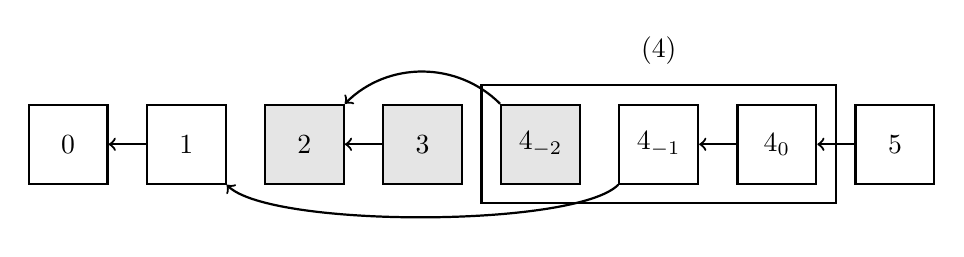
\begin{tikzpicture}[node distance={15mm}, thick, main/.style = {draw, rectangle, minimum size=1cm}]
  \node[main] (0) {0};
  \node[main] (1) [right of=0] {1};
  \node[main,fill=gray!20] (2) [right of=1] {2};
  \node[main,fill=gray!20] (3) [right of=2] {3};
  \node[main,fill=gray!20] (4--2) [right of=3] {$4_{-2}$};
  \node[main] (4--1) [right of=4--2] {$4_{-1}$};
  \node[main] (4-0) [right of=4--1] {$4_0$};
  \node[main] (5) [right of=4-0] {5};
  \draw[->] (1) -- (0);
  \draw[->] (3) -- (2);
  \draw[->] (4--2) to [out=135,in=45,looseness=1] (2);
  \draw[->] (4--1) to [out=225,in=-45,looseness=0.4] (1);
  \draw[->] (4-0) -- (4--1);
  \draw[->] (5) -- (4-0);
  \draw [thick] (5.25,-0.75) rectangle (9.75,0.75);
  \node [label={[shift={(7.5,0.75)}](4)}] {};
  \end{tikzpicture}
  \caption[Dead branch elimination]{Example of applying the dead branch elimination procedure on a proof. Each node represents a proof step or an import; the rectangle represents a subproof step. The nodes in gray are part of dead branches. (3) and ($4_{-1}$) are dead because they are not referenced by any other step. (2) is dead because it is only referenced by (3) and ($4_{-2}$), which are dead. In this situation we can remove the steps (2), (3) along with the import ($4_{-2}$).}
  \label{fig:synthesis-dead-branches}
\end{figure}

\subsubsection{Proof flattening}

A synthesis procedure can make use of subproofs for its own convenience, for instance to dynamically remap premises of an existing proof. Nested subproofs could potentially lead to arbitrarily deep proofs, which is totally valid but can affect the readability and the performances.

This motivates the need of a procedure that can ``flatten'' a proof by inlining all the occurrences of subproofs.


\begin{figure}[H]
  \centering
  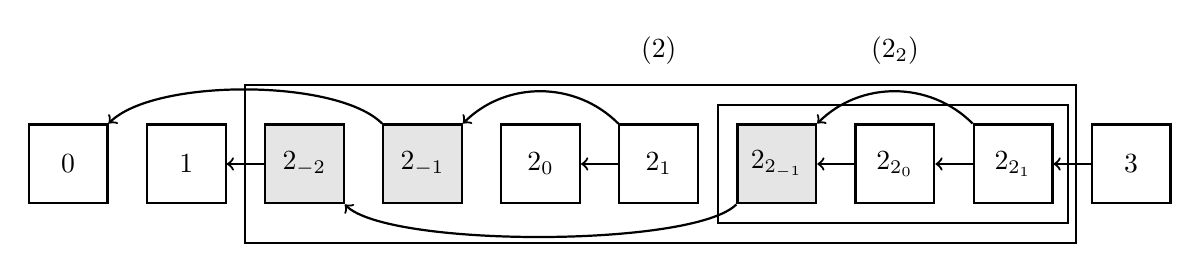
\begin{tikzpicture}[node distance={15mm}, thick, main/.style = {draw, rectangle, minimum size=1cm}]
  \node[main] (0) {0};
  \node[main] (1) [right of=0] {1};
  \node[main,fill=gray!20] (2--2) [right of=1] {$2_{-2}$};
  \node[main,fill=gray!20] (2--1) [right of=2--2] {$2_{-1}$};
  \node[main] (2-0) [right of=2--1] {$2_0$};
  \node[main] (2-1) [right of=2-0] {$2_1$};
  \node[main,fill=gray!20] (2-2--1) [right of=2-1] {$2_{2_{-1}}$};
  \node[main] (2-2-0) [right of=2-2--1] {$2_{2_0}$};
  \node[main] (2-2-1) [right of=2-2-0] {$2_{2_1}$};
  \node[main] (3) [right of=2-2-1] {3};
  \draw[->] (2--2) -- (1);
  \draw[->] (2-1) -- (2-0);
  \draw[->] (2-2-0) -- (2-2--1);
  \draw[->] (2-2-1) -- (2-2-0);
  \draw[->] (3) -- (2-2-1);
  \draw[->] (2--1) to [out=135,in=45,looseness=0.6] (0);
  \draw[->] (2-1) to [out=135,in=45,looseness=1] (2--1);
  \draw[->] (2-2-1) to [out=135,in=45,looseness=1] (2-2--1);
  \draw[->] (2-2--1) to [out=225,in=-45,looseness=0.4] (2--2);
  \draw [thick] (2.25,-1) rectangle (12.8,1);
  \draw [thick] (8.25,-0.75) rectangle (12.7,0.75);
  \node [label={[shift={(7.5,1)}](2)}] {};
  \node [label={[shift={(10.5,1)}]($2_2$)}] {};
  \end{tikzpicture}

  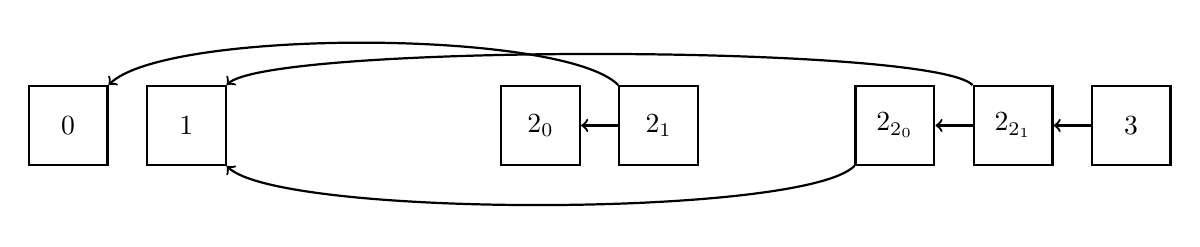
\begin{tikzpicture}[node distance={15mm}, thick, main/.style = {draw, rectangle, minimum size=1cm}]
  \node[main] (0) {0};
  \node[main] (1) [right of=0] {1};
  \node (2--2) [right of=1] {};
  \node (2--1) [right of=2--2] {};
  \node[main] (2-0) [right of=2--1] {$2_0$};
  \node[main] (2-1) [right of=2-0] {$2_1$};
  \node (2-2--1) [right of=2-1] {};
  \node[main] (2-2-0) [right of=2-2--1] {$2_{2_0}$};
  \node[main] (2-2-1) [right of=2-2-0] {$2_{2_1}$};
  \node[main] (3) [right of=2-2-1] {3};
  \draw[->] (2-1) -- (2-0);
  \draw[->] (2-2-0) to [out=225,in=-45,looseness=0.3] (1);
  \draw[->] (2-2-1) -- (2-2-0);
  \draw[->] (3) -- (2-2-1);
  \draw[->] (2-1) to [out=135,in=45,looseness=0.4] (0);
  \draw[->] (2-2-1) to [out=135,in=45,looseness=0.2] (1);
  \end{tikzpicture}
  \caption[Proof flattening]{Example of applying the flattening procedure on a proof. The first graph represents the original proof while the second corresponds to the final state after flattening. The nodes in gray are the imports that have been inlined.}
  \label{fig:synthesis-flattening}
\end{figure}

Every subproof removed contributes to decreasing the size of the proof by one (imports are not counted as proof steps).

In the actual implementation of LISA, the proof checker allows imports to be rewritten. Therefore it is not totally safe to inline proof according to the procedure described above. Instead we need to perform an additional step which is to insert rewrite proof steps for each rewritten import, and use these steps in place of the imports.

\subsubsection{Simplifications}

The previous optimizations ignored the semantics of the LISA sequent calculus. Taking them into account opens up a whole new category of optimization strategies.
For instance, consecutive \code{Rewrite} steps can be merged together assuming the first one of the two is only referenced by other rewrite steps. Similarly, fruitless instantiations can be eliminated and consecutive ones merged in some cases. These optimizations can be represented as a term rewriting system through a set of rules. These rules could in fact be as complex and granular as desired but for the sake of efficiency and because such a procedure is error-prone, we limit ourselves to cases that are likely to be produced by the front. It should be noted that the use of term rewriting rules is a convenient heuristic to approach a generally hard problem: finding the shortest sequent calculus proof in propositional logic is already a hard problem \cite{Krajicek1994}.

The rewriting rules that are currently in place are listed in \autoref{fig:synthesis-simplifications}. We claim that such a system always terminate. For that we introduce a (positive) lexicographic measure for the complexity of the proof where the first criterion is the number of steps and the second one is the sum of of the weights of each step. Rewrite steps have the lowest weights, followed by weakening steps and then all the remaining steps. Then we can see that the measure decreases strictly after any application of a rule, which implies that the system must eventually terminate.

Additionally, if we ignored the cut rules simplifications such a system would be confluent. This follows from the fact that the inputs and outputs are preserved, and that consecutive rewrite/weakening steps can be reduced to a single step in an associative way.

\begin{figure}[H]
  \centering
  \begin{gather*}
  % Any identity
  \begin{prooftree}
  \hypo{\Gamma \vdash \Delta}
  \infer1[$\mathcal{R}$]{\Gamma \vdash \Delta}
  \end{prooftree}
  \quad\leadsto\quad
  \begin{prooftree}
  \hypo{\Gamma \vdash \Delta}
  \end{prooftree} \\[1em]
  % Weakening - Rewrite
  \begin{prooftree}
  \hypo{\Gamma \vdash \Delta}
  \infer1[Weakening]{\Gamma' \vdash \Delta'}
  \end{prooftree}
  \quad\leadsto\quad
  \begin{prooftree}
  \hypo{\Gamma \vdash \Delta}
  \infer1[Rewrite]{\Gamma' \vdash \Delta'}
  \end{prooftree} \\[1em]
  % Rewrite - Rewrite
  \begin{prooftree}
  \hypo{\Gamma \vdash \Delta}
  \infer1[Rewrite]{\Gamma' \vdash \Delta'}
  \infer1[Rewrite]{\Gamma'' \vdash \Delta''}
  \end{prooftree}
  \quad\leadsto\quad
  \begin{prooftree}
  \hypo{\Gamma \vdash \Delta}
  \infer1[Rewrite]{\Gamma'' \vdash \Delta''}
  \end{prooftree} \\[1em]
  % Weakening - Weakening
  \begin{prooftree}
  \hypo{\Gamma \vdash \Delta}
  \infer1[Weakening]{\Gamma', \Gamma \vdash \Delta, \Delta'}
  \infer1[Weakening]{\Gamma'', \Gamma', \Gamma \vdash \Delta, \Delta', \Delta''}
  \end{prooftree}
  \quad\leadsto\quad
  \begin{prooftree}
  \hypo{\Gamma \vdash \Delta}
  \infer1[Weakening]{\Gamma'', \Gamma', \Gamma \vdash \Delta, \Delta', \Delta''}
  \end{prooftree} \\[1em]
  % Rewrite - Weakening
  \begin{prooftree}
  \hypo{\Gamma \vdash \Delta}
  \infer1[Rewrite]{\Gamma' \vdash \Delta'}
  \infer1[Weakening]{\Gamma'', \Gamma' \vdash \Delta', \Delta''}
  \end{prooftree}
  \quad\leadsto\quad
  \begin{prooftree}
  \hypo{\Gamma \vdash \Delta}
  \infer1[Weakening]{\Gamma'', \Gamma' \vdash \Delta', \Delta''}
  \end{prooftree} \\[1em]
  % Weakening - Rewrite
  \begin{prooftree}
  \hypo{\Gamma \vdash \Delta}
  \infer1[Weakening]{\Gamma', \Gamma \vdash \Delta, \Delta'}
  \infer1[Rewrite]{\Gamma'' \vdash \Delta''}
  \end{prooftree}
  \quad\leadsto\quad
  \begin{prooftree}
  \hypo{\Gamma \vdash \Delta}
  \infer1[Weakening]{\Gamma'' \vdash \Delta''}
  \end{prooftree} \\[1em]
  % Hypothesis - Rewrite
  \begin{prooftree}
  \hypo{}
  \infer1[Hypothesis]{\Gamma, \phi \vdash \phi, \Delta}
  \infer1[Rewrite]{\Gamma', \phi \vdash \phi, \Delta'}
  \end{prooftree}
  \quad\leadsto\quad
  \begin{prooftree}
  \hypo{}
  \infer1[Hypothesis]{\Gamma', \phi \vdash \phi, \Delta'}
  \end{prooftree} \\[1em]
  % Hypothesis - Weakening
  \begin{prooftree}
  \hypo{}
  \infer1[Hypothesis]{\Gamma, \phi \vdash \phi, \Delta}
  \infer1[Weakening]{\Gamma', \Gamma, \phi \vdash \phi, \Delta, \Delta'}
  \end{prooftree}
  \quad\leadsto\quad
  \begin{prooftree}
  \hypo{}
  \infer1[Hypothesis]{\Gamma', \Gamma, \phi \vdash \phi, \Delta, \Delta'}
  \end{prooftree} \\[1em]
  % Cut left
  \begin{prooftree}
  \hypo{\Gamma_1 \vdash \phi, \Delta_1}
  \hypo{\Gamma_2, \phi \vdash \Delta_2}
  \infer2[Cut]{\Gamma_1, \Gamma_2, \phi \vdash \Delta_1, \Delta_2}
  \end{prooftree}
  \quad\leadsto\quad
  \begin{prooftree}
  \hypo{\Gamma_2, \phi \vdash \Delta_2}
  \infer1[Weakening]{\Gamma_1, \Gamma_2, \phi \vdash \Delta_1, \Delta_2}
  \end{prooftree} \\[1em]
  % Cut right
  \begin{prooftree}
  \hypo{\Gamma_1 \vdash \phi, \Delta_1}
  \hypo{\Gamma_2, \phi \vdash \Delta_2}
  \infer2[Cut]{\Gamma_1, \Gamma_2 \vdash \phi, \Delta_1, \Delta_2}
  \end{prooftree}
  \quad\leadsto\quad
  \begin{prooftree}
  \hypo{\Gamma_1 \vdash \phi, \Delta_1}
  \infer1[Weakening]{\Gamma_1, \Gamma_2 \vdash \phi, \Delta_1, \Delta_2}
  \end{prooftree}
  \end{gather*}
  \caption[Term rewriting rules]{Term rewriting rules used to simply a proof. The first rule states that any proof step with one hypothesis equal to the conclusion can be suppressed.}
  \label{fig:synthesis-simplifications}
\end{figure}
